\chapter{Realisierungsfahrplan}

Die Erstellung des Realisierungsfahrplans wurde im Team vorgenommen.
Hierbei wurden Aufgaben mit entsprechenden Unteraufgaben definiert und die geschätzen Zeiten eingtragen.
Die Darstellung des Realisierungsfahrplans erfolgte als Gantt-Diagramm, welches auf der nächsten Seite abgebildet ist.
Das Diagramm zeigt die Aufgaben bis zur Fertigstellung der ersten Version der App (``V1'').

Das Gantt-Diagramm zeigt den kritischen Pfad (rot eingefärbt) auf.
Dieser erstreckt sich vom Entwurf der Softwarearchitektur bis hin zum Upload der App in den App-Store.
Der kritische Pfad ergibt sich zum einen aus der langen Implementierungszeit, zum anderen können weitere Aufgaben (vollständiger Systemtest, Upload in die Stores) erst dann erfolgen, wenn die Entwicklung vollständig abgeschlossen ist.
Dies wirkt sich somit auf das Enddatum aus, an welchem die App in den Stores verfügbar sein wird.

Bereits bei früheren Projekten wurde die Erfahrung gemacht, dass der Upload in Apple's App-Store länger dauert als ein Upload im Google-Play-Store. Der Grund hierfür liegt bei den manuellen App-Tests, die von Mitarbeitern des Unternehmens Apple durchgeführt werden. Erst wenn sie die App akzeptieren, wird sie im Store zum Download bereitgestellt. \\

Bei der Realisierungsplanung wurden folgende Meilensteine festgelegt:
\begin{description}[leftmargin=!,labelwidth=\widthof{\bfseries KONZEPTION APP UI}]
\item [KONZEPTION APP-UI] Dieser Meilenstein ist erreicht, wenn das Oberflächendesign für die App vollständig entworfen wurde.
\item [WEBSEITE LIVE] Dieser Meilenstein ist erreicht, wenn die Homepage von \textit{Imagical} online zugänglich ist.
\item [APP V1] Dieser Meilenstein ist erreicht, wenn die Entwicklungsarbeiten für die erste Version der App abgeschlossen sind.
\item [APP ONLINE] Dieser Meilenstein ist erreicht, wenn die App in beiden App-Stores verfügbar ist.
\end{description}

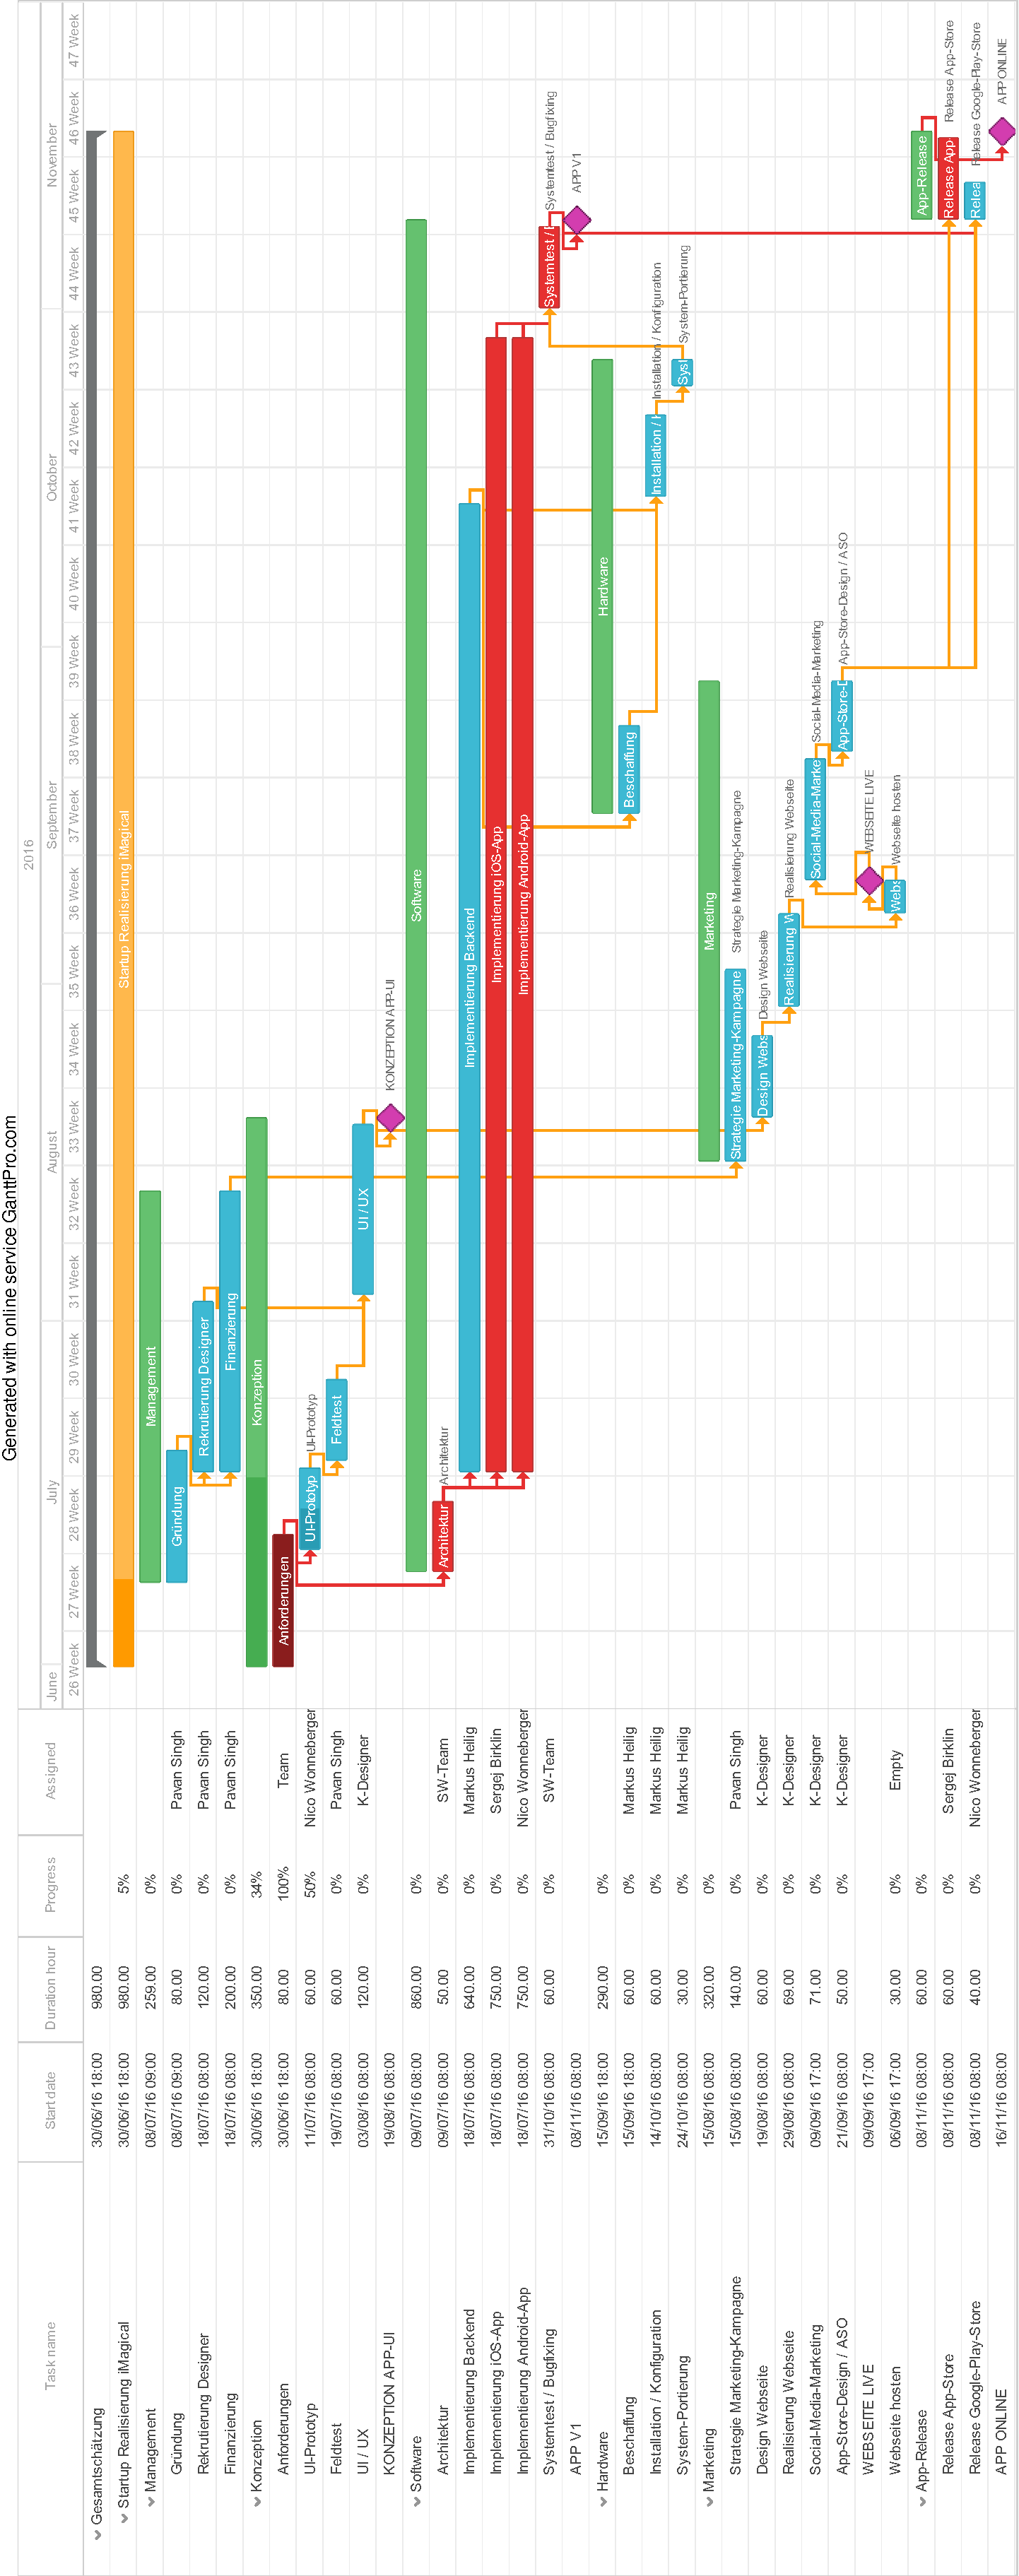
\includepdf{assets/gantt} 
